% !TEX encoding = UTF-8 Unicode 
% !TEX root = praca.tex

\chapter*{Metodyka badań}

\section*{Przygotowanie środowiska}

Do przeprowadzenia eksperymentów z wybranymi metodami XAI wymagane było odpowiednie przygotowanie środowiska programistycznego.
W tej pracy wykorzystano  następujące narzędzia i biblioteki:
\begin{itemize}
	\item \textbf{Python} - wysokopoziomowy język programowania, który jest szeroko stosowany w dziedzinie nauki o danych i uczenia maszynowego.
	      Był to główny język używany w badaniach.
	\item \textbf{TensorFlow} - popularna biblioteka open-source do uczenia maszynowego, która jest szeroko stosowana w dziedzinie uczenia maszynowego do tworzenia i trenowania modeli głębokich.
	\item \textbf{LIME} - biblioteka do generowania lokalnie interpretowalnych wyjaśnień dla decyzji modelu.
	\item \textbf{SHAP} - biblioteka oparta na teorii gier, która oblicza wartości Shapleya, określająca wpływ poszczególnych cech na wynik modelu.
	\item \textbf{numpy} - szeroko stosowana biblioteka do obliczeń numerycznych.
	\item \textbf{matplotlib} - biblioteka do tworzenia wykresów i wizualizacji danych, szeroko stosowana w dziedzinie uczenia maszynowego.
	\item \textbf{scikit-image} - biblioteka do przetwarzania obrazów, która zawiera wiele funkcji do przetwarzania obrazów.
	\item \textbf{Pandas} - biblioteka do manipulacji i analizy danych, które oferuje struktury danyc hi narzędzia do przetwarzania danych tabelarycznych.
	      Szczególnie użyteczna do zarządzania i analizowania zbiorów danych używanych w badaniach.
	\item \textbf{seabron} - biblioteka do tworzenia wykresów i wizualizacji danych, współgrająca z biblioteką pandas
\end{itemize}
Środowisko to pozwoliło na tworzenie i analizowanie wyjaśnień dla już istniejących modeli głębokiego uczenia.
Narzędzia te umożłiwiły także wizualizację wyników, co było kluczowe dla zrozumienia i prezentacji działania zastosowanych metod XAI.

Dodatkowo, wykorzystano baza danych \textbf{ImageNet-9} jest to podzbiór ImageNet który zawiera 9 kategorii, z których każda posiada 450 obrazów.
Baza ta zawietała również oznaczone przez ekspertów obszary obiektów klasyfikowanych, co pozwalało na posiadanie wiedzy o ważnych obszarach.
Kategorie obejmowały:
\begin{itemize}
	\item Pies (dog)
	\item Ptak (bird)
	\item Pojazd na kółkach (wheeled vehicle)
	\item Gad (reptile)
	\item Mięsożerca (carnivore)
	\item Insekt (insect)
	\item Instrumenty muzyczne (musical instrument)
	\item Naczelny (primate)
	\item Ryba (fish)
\end{itemize}

\section*{Podział na rozmiar obiektu}

Obrazy z bazy danych zostały podzielone ze względu na procent jaki obszaru zajmowanego przez obiekt docelowy.
Zostały stworzone 3 kategorie obrazów:
\begin{itemize}
	\item Mały - obiekt zajmuje 25\% obrazu lub mniej
	\item Średni - obiekt zajumuje 50\% obrazu lub mniej, ale więcej niż 25\% obrazu
	\item Duży - obiekt zajmuje więcej niż 50\% obrazu
\end{itemize}

W tej pracy w kategorii małe znajduje się 1347 obrazów, w kategorii średnie znajduje się 1437 obrazów oraz w kategorii duże znajduje się 1266 obrazów.

\begin{figure}
	\centering
	\begin{subfigure}[b]{0.3\textwidth}
		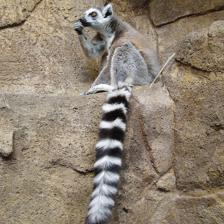
\includegraphics[width=.9\textwidth]{img/examples/size_category_small}
		\caption{Mały obiekt (0.7553\%)}  \label{}
	\end{subfigure}
	\begin{subfigure}[b]{0.3\textwidth}
		\centering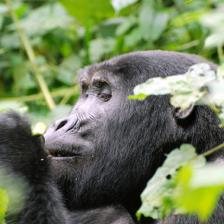
\includegraphics[width=.9\textwidth]{img/examples/size_category_medium}
		\caption{Średni obiekt (35.8897\%)}  \label{}
	\end{subfigure}
	\begin{subfigure}[b]{0.3\textwidth}
		\centering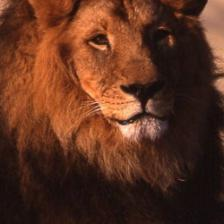
\includegraphics[width=.9\textwidth]{img/examples/size_category_big}
		\caption{Duży obiekt (97.1939\%)}  \label{}
	\end{subfigure}
	\caption{Przykłady obrazów dla różnych kategori wielkości}
\end{figure}

\section*{Wybór parametrów metod XAI}
Wybór odopwiednich parametrów jest kluczowym etapem w procesie tworzenia i oceny modeli głębokiego uczenia oraz metod wyjaśnialnej sztucznej inteligencji (XAI).
Parametry mają bezpośredni wpływ na jakość, dokładność i interpretowalność wyników generowanych przez modele i metody XAI.
W tej sekcji omówione zostało, jakie parametry zostały wybrane dla każdej z zastosowanych metod (LIME, SHAP i GradCAM), oraz jak te parametry wpływają na wyniki i interpretacje uzyskane w badaniach

\subsection*{LIME}
W celu porównania metod na większej liczbie obrazów konieczne było ustalenie wartości parametrów dla poszczególnych technik.
W bibliotece LIME używamy tych parametrów LIME:
\begin{itemize}
	\item \textbf{num samples}
	\item \textbf{num features}
	\item \textbf{possitive only}
	\item \textbf{min weight}
\end{itemize}

Parametr \textbf{'num\_samples'} to liczba próbek generowanych wokół wyjaśnianej instancji.
Wyjaśnienia LIME opierają się na lokalnych modelach zastępczych, które są trenowane na perturbowanych wersjach oryginalnych danych wejściowych.
Zbyt mała liczba próbek może prowadzić do niedokładnych wyjaśnień, ponieważ lokalny model zastępczy może nie być w stanie prawidłowo uchwycić istotnych wzorców w danych.
Z drugiej strony, zbyt duża liczba próbek może prowadzić do znacznych kosztów obliczeniowych, co wydłuża czas potrzebny na wygenerowanie wyjaśnień.
W tej pracy użyto wartości num\_samples=1000, co stanowi kompromis między dokładnością wyjaśnień a kosztami obliczeniowymi.

\begin{figure}
	\centering
	\begin{subfigure}[b]{0.3\textwidth}
		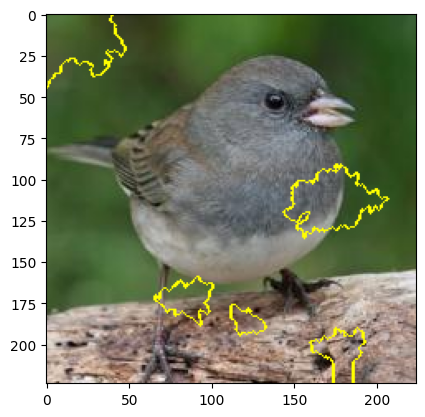
\includegraphics[width=.9\textwidth]{img/parameters/lime/num_samples_5}
		\caption{num\_samples=5}  \label{rys:parameters_lime_numsamples_5}
	\end{subfigure}
	\begin{subfigure}[b]{0.3\textwidth}
		\centering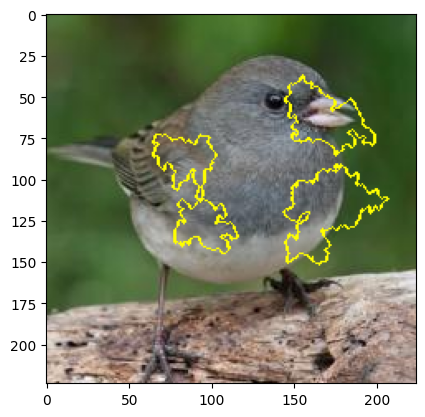
\includegraphics[width=.9\textwidth]{img/parameters/lime/num_samples_1000}
		\caption{num\_samples 1000}  \label{rys:parameters_lime_numsamples_1000}
	\end{subfigure}
	\begin{subfigure}[b]{0.3\textwidth}
		\centering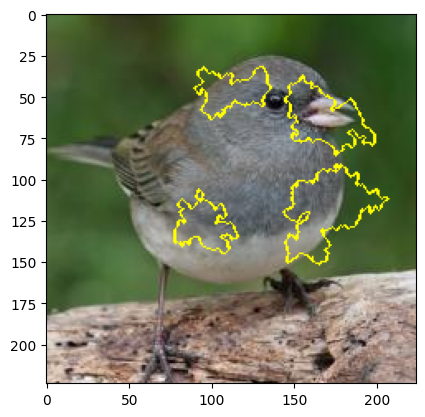
\includegraphics[width=.9\textwidth]{img/parameters/lime/num_samples_5000}
		\caption{num\_samples 5000}  \label{rys:parameters_lime_numsamples_5000}
	\end{subfigure}
	\caption{Przykłady wyjaśnień LIME dla różnych wartości num\_samples}
\end{figure}

Parametr \textbf{'num\_features'} oznacza maksymalną ilość cech które mogą występować w wyjaśnieniu.
Wyjaśnienia LIME polegają na identyfikacji najważniejszych cech, które wþływają na decyzję modelu w danym punkcie.
W przypadku obrazów, cech te są reprezentowane przez superpiksele, czyli segmenty obrazu zawierające grupy pikseli.
Określenie zbyt niskiej wartości dla num\_features może prowadzić do pominięcia istotnych cech, co skutkuje niepełnym wyjaśnieniem.
Z kolei zbyt wysoka wartość może sprawić, że wyjaśnienie będzie zawerało nadmiarowe informacje, które mogą być trudnę do interpretacji.

W przypadku tej pracy, ponieważ obraz jest dzielony na części (superpiksele), nawet duża wartość parametru num\_features daje stosunkowo małą ilość cech.
Użytwo dużej wartości, aby nie ominąć żadnych istotnych cech.
Dlatego w tej pracy pozostawiono domyślną wartość num\_features = 100000, aby zapewnić, że wszystkie potencjalnie ważne cechy zostaną uwzględnione w wyjaśnieniach.

\begin{figure}
	\centering
	\begin{subfigure}[b]{0.3\textwidth}
		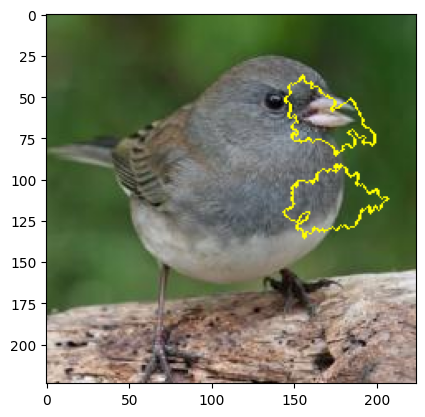
\includegraphics[width=.9\textwidth]{img/parameters/lime/num_features_2}
		\caption{num\_features 2}  \label{rys:parameters_lime_numsamples_5}
	\end{subfigure}
	\begin{subfigure}[b]{0.3\textwidth}
		\centering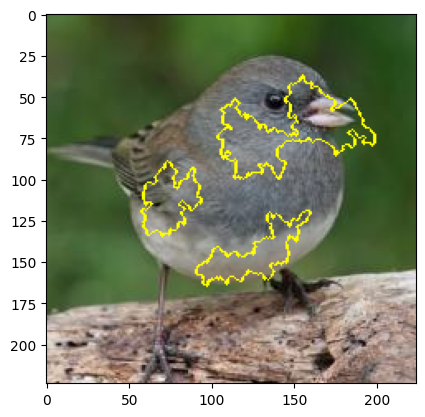
\includegraphics[width=.9\textwidth]{img/parameters/lime/num_features_100000}
		\caption{num\_features 100000}  \label{rys:parameters_lime_numsamples_1000}
	\end{subfigure}
	\caption{Przykłady wyjaśnień LIME dla różnych wartości num\_features}
\end{figure}

Parametr \textbf{'positive\_only'} określa, czy wyjaśnienia powinny uwzględniać tylko cechy, które mają pozytywny wpływ na klasyfikację.
Ustawienie tego parametru na prawdziwy pomaga w identyfikowaniu pozytywnych cech, które wpływają na decyzję modelu.
Natomiast ustawienie tego parametru na prawdziwy pomaga w identyfikowaniu także negatywnych cech.
Ta praca skupia się na wyjaśnianiu dlaczego model podją daną decyzję więc parametr \textbf{positive\_only} jest ustawiony na prawdziwy.

Parametr \textbf{min\_weight} określa minimalną wagę cech, która musi być spełniona, aby cecha była uwzględniona w wyjaśnieniu.
Ustawienie wartości na 0.0 oznacza, że wszystkie cechy będą brane pod uwagę, niezależnie od ich wpływu na decyzję modelu.
W praktyce jednak, zbyt duża liczba cech może skomplikować wyjaśnienia i uczynić je trudniejszymi do interpretacji.
Dlatego w niektórych przypadkach może być użyteczne ustawienie tej wartości na wyższą, aby uwzględniać tylko te cechy, które mają istotny wpływ na wynik.
W tej pracy ustawiono min\_weight na 0.0, aby uwzględnić wszystkie cechy w wyjaśnieniach.

\begin{figure}
	\centering
	\begin{subfigure}[b]{0.3\textwidth}
		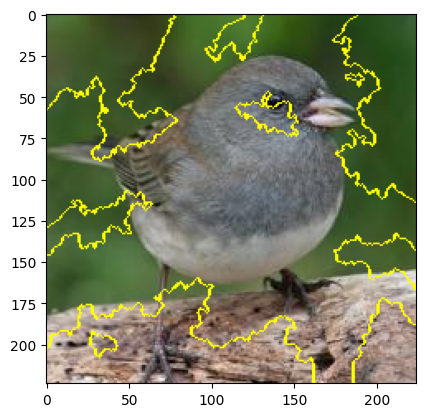
\includegraphics[width=.9\textwidth]{img/parameters/lime/min_weight_00}
		\caption{min\_weight 0.0}  \label{rys:parameters_lime_numsamples_5}
	\end{subfigure}
	\begin{subfigure}[b]{0.3\textwidth}
		\centering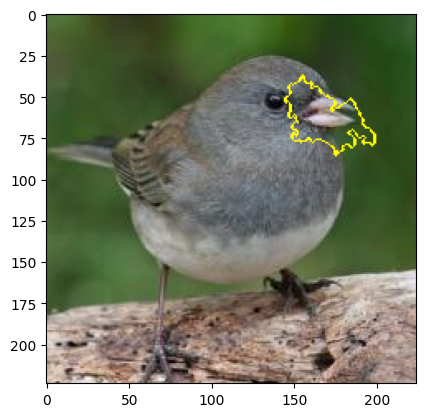
\includegraphics[width=.9\textwidth]{img/parameters/lime/min_weight_03}
		\caption{min\_weight 0.3}  \label{rys:parameters_lime_numsamples_1000}
	\end{subfigure}
	\caption{Przykłady wyjaśnień LIME dla różnych wartości min\_weight}
\end{figure}


\subsection*{SHAP}
Analogicznie do metody LIME, musimy ustalić odpowiednie parametry dla metody SHAP.
Parametry mają kluczowe znaczenie dla uzyskania dokładnych i interpretowalnych wyjaśnień.
W przypadku metody SHAP, wybrano dwa główne parametry:
\begin{itemize}
	\item \textbf{max\_evals}
	\item \textbf{threshold}
\end{itemize}

Parametr max\_evals to liczba maksymalnych ewaluacji modelu, które mogą być wykonane w celu obliczenia wartości SHAP.
Wartość ta ma bezpośredni wpływ na jakość i dokładność wyjaśnień.
Wyższa liczba ewaluacji zazwyczaj prowadzi do bardziej precyzyjnych wyników, ponieważ pozwala na lepsze oszacowanie wpływu poszczególnych cech na wynik modelu.
Jednakże, zwiększenie wartości max\_evals wiąże się również ze zwiększonymi kosztami obliczeniowymi, co może być istotne przy analizie dużych zbiorów danych lub skomplikowanych modeli.

W tej pracy ustaliliśmy wartość max\_evals na 500, co stanowi kompromis pomiędzy dokładnością wyjaśnień a czasem potrzebnym na ich obliczenie.

\begin{figure}
	\centering
	\begin{subfigure}[b]{0.45\textwidth}
		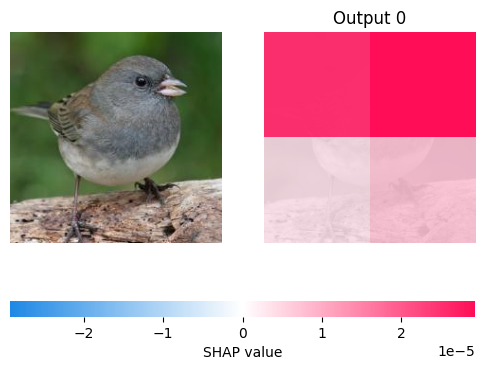
\includegraphics[width=.9\textwidth]{img/parameters/shap/max_evals_10}
		\caption{max\_evals 10}  \label{rys:parameters_lime_numsamples_5}
	\end{subfigure}
	\begin{subfigure}[b]{0.45\textwidth}
		\centering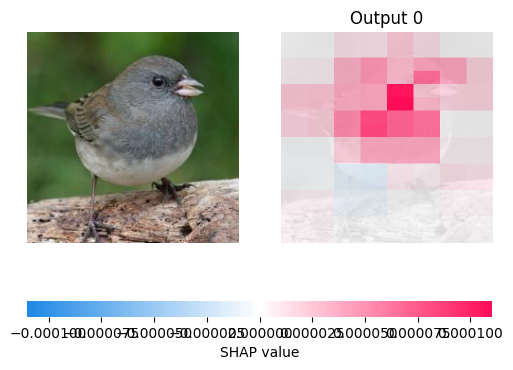
\includegraphics[width=.9\textwidth]{img/parameters/shap/max_evals_500}
		\caption{max\_evals 500}  \label{rys:parameters_lime_numsamples_1000}
	\end{subfigure}
	\caption{Przykłady wyjaśnienia SHAP dla parametru max\_evals}
\end{figure}
Parametr \textbf{threshold} określa minimalną wartość cechy, która musi być spełniona, aby cecha została uwzględniona w wyjaśnieniu.
Wartość progowa jest ważna, ponieważ pozwala na filtrowanie mniej istotnych cech, co może uprościć wyjaśnienia i uczynić je bardziej zrozumiałymi.
W przypadku obrazów, gdzie liczba cech jest bardzo duża, odpowiednie ustawienie tego parametru jest kluczowe.

W tej pracy ustaliliśmy wartość threshold jako średnią wartość cechy dla danego obrazu.
Parametr ten został stworzony, aby umożliwić porównywanie różnych metod wyjaśniania.
Threshold pełni kluczową rolę w procesie modyfikacji zbioru cech wyjaśnień.
Względem tego parametru, wybierane są tylko te cechy, których wartości są większe lub równe średniej wartości cech.
Dzięki temu mechanizmowi, wyjaśnienia koncentrują się na cechach, które mają znaczący wpływ na decyzję modelu, eliminując te, które mają minimalny wpływ.
W efekcie, wyjaśnienia stają się bardziej skoncentrowane na kluczowych cechach decyzyjnych.
\begin{equation}
	\hat{E} =  \{ e_i \in E \mid e_i \geq \frac{1}{|E|}\sum_{i=1}^{|E|} e_i \}
	\label{eq:modified_explanation}
\end{equation}
Gdzie:
\begin{itemize}[label=]
	\item $\hat{E}$ to zbiór zmodyfikowanych wartości cech wyjaśnień
	\item $\text{E}$ to oryginalny zbiór wartości cech wyjaśnień
\end{itemize}

\begin{figure}
	\centering
	\begin{subfigure}[b]{0.45\textwidth}
		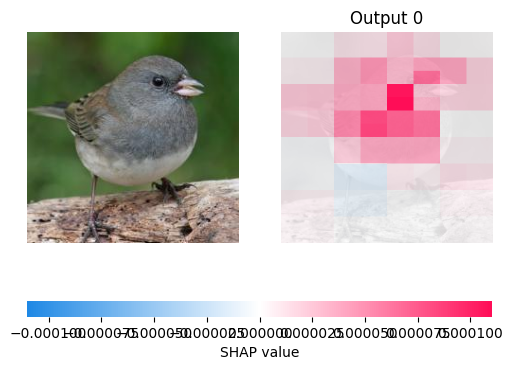
\includegraphics[width=.9\textwidth]{img/parameters/shap/threshold_base}
		\caption{Orginalne wyjaśnienie}  \label{rys:parameters_lime_numsamples_5}
	\end{subfigure}
	\begin{subfigure}[b]{0.45\textwidth}
		\centering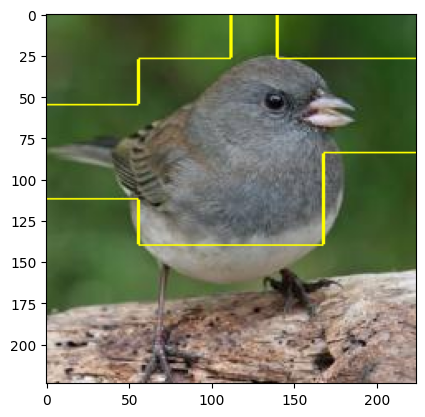
\includegraphics[width=.9\textwidth]{img/parameters/shap/threshold_mean}
		\caption{Zmodyfikowane wyjaśnienie}  \label{rys:parameters_lime_numsamples_1000}
	\end{subfigure}
	\caption{Przykład modyfikowania wyjaśnienia SHAP za pomocą threshold}
\end{figure}

\subsection*{GradCAM}
W przypadku metody GradCAM również musimy skonfigurować parametr "threshold", który pozwoli nam porównać różne wyjaśnienia generowane przez tę metodę.
Parametr ten jest istotny dla procesu modyfikacji wyjaśnień, podobnie jak miało to miejsce w przypadku metody SHAP.
Wartość "threshold" w metodzie GradCAM określa minimalną wartość pikseli, które będą uwzględnione w wyjaśnieniu.
Im wyższa wartość threshold, tym mniej pikseli zostanie uwzględnionych, co może prowadzić do bardziej skupionych wyjaśnień na kluczowych obszarach obrazu.
Z kolei niższa wartość threshold może uwzględnić więcej pikseli, co może prowadzić do bardziej rozproszonych wyjaśnień.

Wybrana została wartoś cthreshold na poziomie 0.2.
\begin{equation}
	\hat{E} =  \{ e_i \in E \mid e_i \geq 0.2 \}
	\label{eq:modified_explanation_gradcam}
\end{equation}
Gdzie:
\begin{itemize}[label=]
	\item $\hat{E}$ to zbiór zmodyfikowanych wartości cech wyjaśnień
	\item $\text{E}$ to oryginalny zbiór wartości cech wyjaśnień
\end{itemize}

\begin{figure}
	\centering
	\begin{subfigure}[b]{0.9\textwidth}
		\centering
		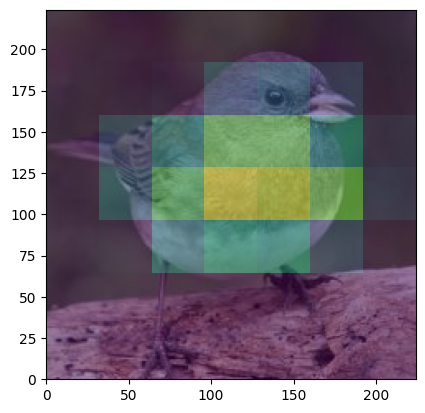
\includegraphics[width=.45\textwidth]{img/parameters/gradcam/threshold_base}
		\caption{Orginalne wyjaśnienie}  \label{rys:parameters_lime_numsamples_5}
	\end{subfigure}
	\begin{subfigure}[b]{0.45\textwidth}
		\centering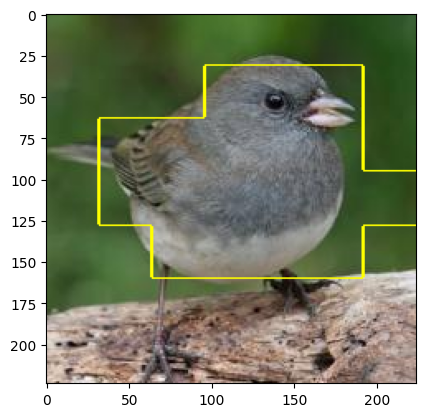
\includegraphics[width=.9\textwidth]{img/parameters/gradcam/threshold_01}
		\caption{Threshold 0.1}  \label{rys:parameters_lime_numsamples_1000}
	\end{subfigure}
	\begin{subfigure}[b]{0.45\textwidth}
		\centering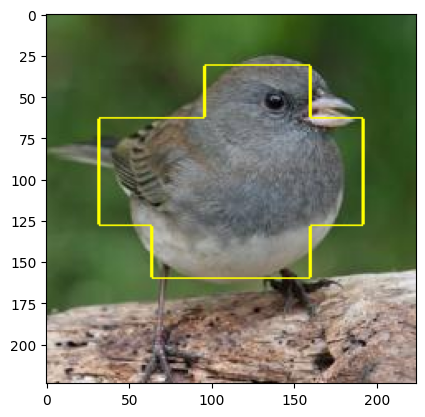
\includegraphics[width=.9\textwidth]{img/parameters/gradcam/threshold_02}
		\caption{Threshold 0.2}  \label{rys:parameters_lime_numsamples_1000}
	\end{subfigure}
	\begin{subfigure}[b]{0.45\textwidth}
		\centering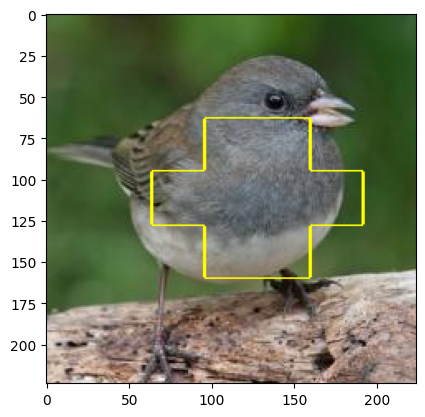
\includegraphics[width=.9\textwidth]{img/parameters/gradcam/threshold_05}
		\caption{Threshold 0.5}  \label{rys:parameters_lime_numsamples_1000}
	\end{subfigure}
	\begin{subfigure}[b]{0.45\textwidth}
		\centering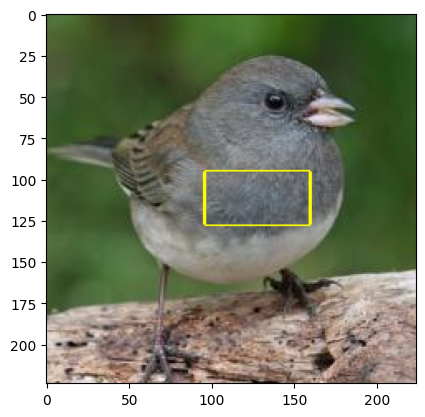
\includegraphics[width=.9\textwidth]{img/parameters/gradcam/threshold_09}
		\caption{Threshold 0.9}  \label{rys:parameters_lime_numsamples_1000}
	\end{subfigure}
	\caption{Przykład modyfikowania wyjaśnień GradCAM za pomocą threshold}

\end{figure}

\subsection*{Łączenie wyjaśnień}

Wyjaśnienia możemy łączyć na 2 różne sposoby:
\begin{itemize}
	\item Część wspólna obszarów wyjaśnień - bardziej szczegółowe wyjaśnienia
	\item Suma obszarów wyjaśnień - bardziej ogólne wyjaśnienia
\end{itemize}

\begin{figure}
	\centering
	\begin{subfigure}[b]{0.45\textwidth}
		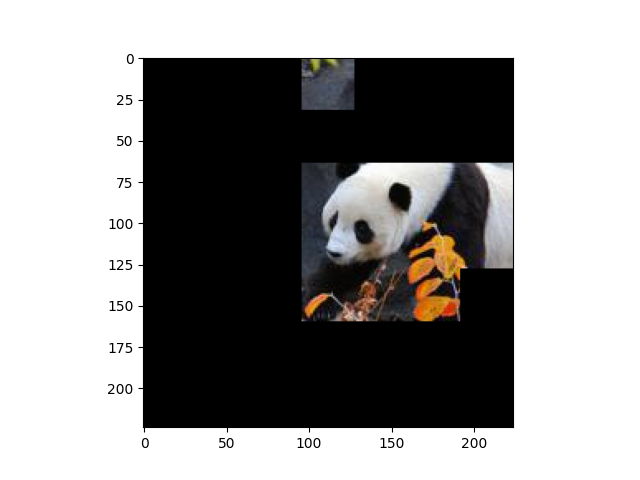
\includegraphics[width=.9\textwidth]{img/examples/first_explanation}
		\caption{Wyjaśnienie GradCAM}  \label{}
	\end{subfigure}
	\begin{subfigure}[b]{0.45\textwidth}
		\centering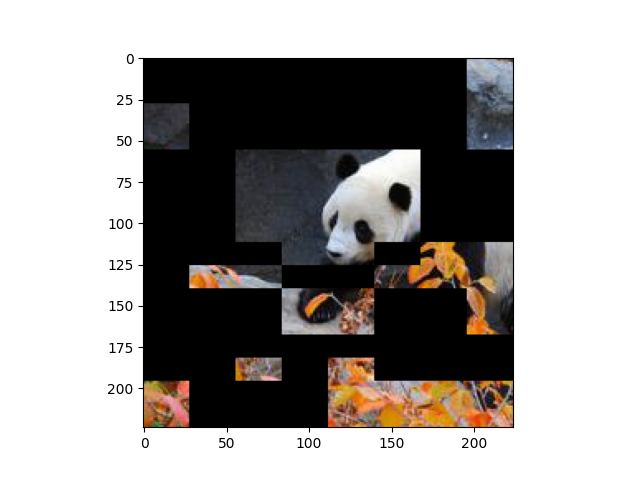
\includegraphics[width=.9\textwidth]{img/examples/second_explanation}
		\caption{Wyjaśnienie SHAP}  \label{}
	\end{subfigure}
	\begin{subfigure}[b]{0.45\textwidth}
		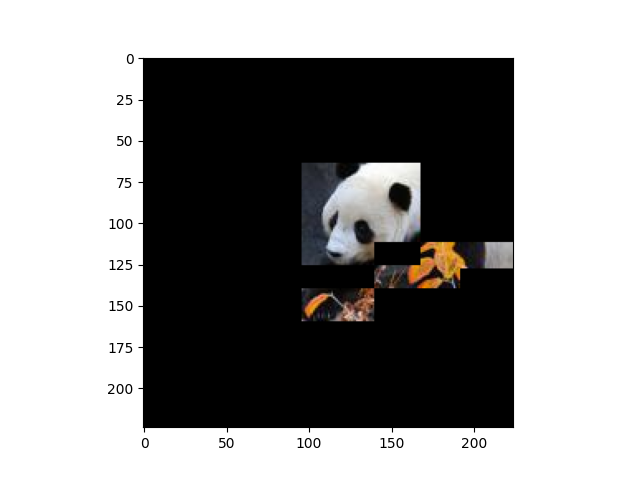
\includegraphics[width=.9\textwidth]{img/examples/and_explanation}
		\caption{Część wspólna wyjaśnień}  \label{}
	\end{subfigure}
	\begin{subfigure}[b]{0.45\textwidth}
		\centering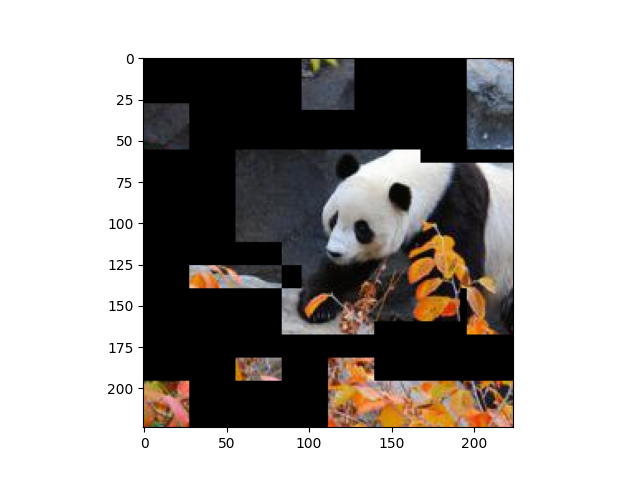
\includegraphics[width=.9\textwidth]{img/examples/or_explanation}
		\caption{Suma obszarów wyjaśnień}  \label{}
	\end{subfigure}
	\caption{Przykład łączenia wyjaśnień} \label{rys:test}
\end{figure}

\section*{Miary jakości}

W tej sekcji skupiano się na opisie miar jakości, które zostały wykorzystane do oceny skuteczności metod wyjaśnialnej sztucznej inteligencji (XAI) w kontekście zadania klasyfikacji obrazów.

Wskaźnik \textbf{IoU} (Intersection ober Union), czyli stosunek przecięcia do sumy, jest powszechnie stosowany do pomiaru stopnia nakładania się dwóch obszarów.
W kontekście XAI, IoU jest używany do porównywania obszaru wyjaśnienia z obszarem rzeczywistego obiektu lub regionu zainteresowania na obrazie.
Im wyższy IoU, tym lepiej wyjaśnienie pokrywa się z rzeczywistym obiektem na obrazie.

Miara \textbf{Zmiana pewności dla samego obszaru wyjaśnienia} ocenia, jak zmienia się pewność modelu, gdy pozostawiony zostaje jedynie obszar wyjaśnienia.
Im lepsze wyjaśnienie, tym mniejszy średni spadek pewności. Pewność modelu może również wzrosnąć, jeśli pozostaną tylko istotne obszary.
Innymi słowy, im lepsze wyjaśnienie, tym większy procent przypadków, w których pewność modelu wzrosła po pozostawieniu obszaru wyjaśnienia.

\begin{figure}
	\begin{subfigure}[b]{0.45\textwidth}
		\centering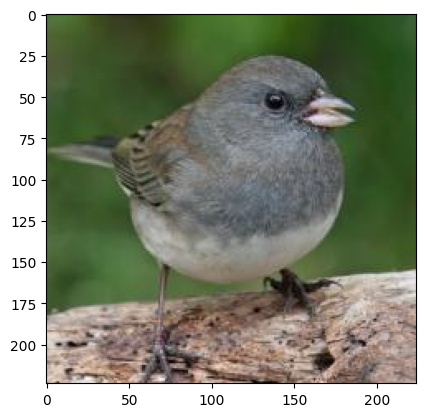
\includegraphics[width=.9\textwidth]{img/parameters/quality/base}
		\caption{Orginalny obraz}  \label{rys:parameters_lime_numsamples_1000}
	\end{subfigure}
	\begin{subfigure}[b]{0.45\textwidth}
		\centering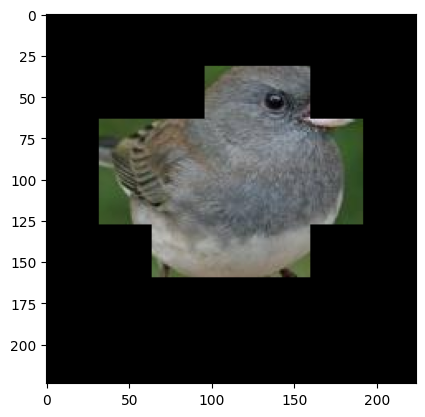
\includegraphics[width=.9\textwidth]{img/parameters/quality/mask}
		\caption{Sam obszar wyjaśnienia}  \label{rys:parameters_lime_numsamples_1000}
	\end{subfigure}
	\caption{Przykład pozostawienia samego wyjaśnienia}
\end{figure}

Miara \textbf{Zmiana pewności dla braku obszaru wyjaśnienia} ocenia, jak zmienia się pewność modelu, gdy usunięty zostaje obszar wyjaśnienia.
Im lepsze wyjaśnienie, tym większy średni spadek pewności.

\begin{figure}
	\begin{subfigure}[b]{0.45\textwidth}
		\centering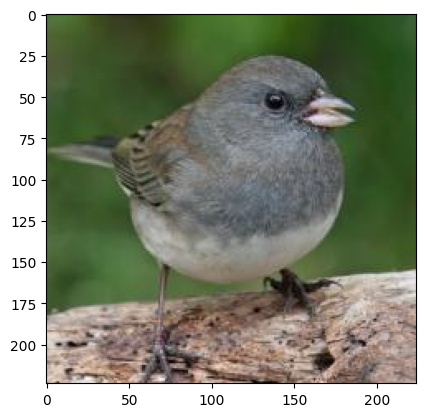
\includegraphics[width=.9\textwidth]{img/parameters/quality/base}
		\caption{Orginalny obraz}  \label{rys:parameters_lime_numsamples_1000}
	\end{subfigure}
	\begin{subfigure}[b]{0.45\textwidth}
		\centering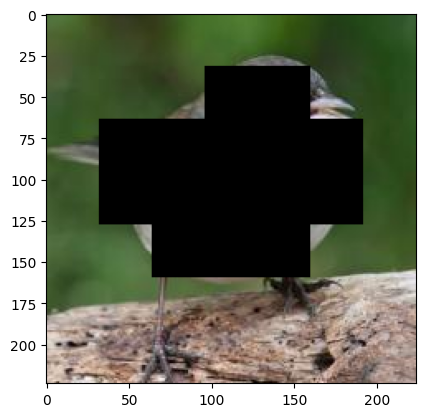
\includegraphics[width=.9\textwidth]{img/parameters/quality/wo_mask}
		\caption{Obraz bez obszaru wyjaśnienia}  \label{rys:parameters_lime_numsamples_1000}
	\end{subfigure}
	\caption{Przykład usunięcia obszaru wyjaśnienia}
\end{figure}

\section*{Plan badań}

\begin{itemize}
	\item Skonfigurowanie środowiska pracy, w tym odpowiednie biblioteki Pythona.
	\item Załadowanie zbioru danych, który będzie używany do testowania metod wyjaśniania XAI.
	\item Przygotowanie modelu klasyfikacji obrazów, który będzie poddany analizie.
	\item \textbf{Dobór parametrów}:
	      \begin{itemize}
		      \item Określenie optymalnych wartości parametrów dla każdej z metod wyjaśniania, takich jak liczba próbek dla LIME, czy liczba iteracji dla SHAP.
		      \item Przeprowadzenie eksperymentów w celu znalezienia optymalnych ustawień parametrów dla każdej metody.
	      \end{itemize}

	\item \textbf{Wygenerowanie wyjaśnień}:
	      \begin{itemize}
		      \item Wygenerowanie wyjaśnień dla wszystkich obrazów ze zbioru danych za pomocą wybranych metod XAI.
		      \item Zapisanie uzyskanych wyjaśnień dla dalszej analizy.
	      \end{itemize}

	\item \textbf{Wykonanie podstawowych badań na wszystkich obrazach}:
	      \begin{itemize}
		      \item Zastosowanie wybranych miar jakości, takich jak IoU, w celu oceny skuteczności każdej metody wyjaśniania.
		      \item Analiza wyników pod kątem różnych kryteriów, takich jak pokrycie obszarów istotnych dla decyzji modelu.
	      \end{itemize}

	\item \textbf{Wykonanie badań grupując na kategorie}:
	      \begin{itemize}
		      \item Podział obrazów na kategorie na podstawie określonych cech, takich jak klasa obiektów czy złożoność sceny.
		      \item Analiza skuteczności metod wyjaśniania w poszczególnych kategoriach i porównanie wyników.
	      \end{itemize}

	\item \textbf{Wykonanie badań biorąc pod uwagę pewność modelu}:
	      \begin{itemize}
		      \item Ocena wpływu pewności modelu na skuteczność metod wyjaśniania, w tym analiza zmian pewności w zależności od obszaru wyjaśnienia.
		      \item Porównanie wyników uzyskanych dla różnych poziomów pewności modelu.
	      \end{itemize}

	\item \textbf{Wykonanie podstawowych badań dla innego modelu}:
	      \begin{itemize}
		      \item Przetestowanie metod wyjaśniania na innym modelu klasyfikacji obrazów.
		      \item Porównanie wyników uzyskanych dla różnych modeli i ocena ich zgodności.
	      \end{itemize}

	\item \textbf{Wykonanie podstawowych badań dla specyficznych klas}:
	      \begin{itemize}
		      \item Skoncentrowanie się na analizie wyjaśnień dla konkretnych klas obiektów lub zjawisk.
		      \item Ocena, czy metody wyjaśniania są skuteczne w wykrywaniu istotnych cech dla określonych klas.
	      \end{itemize}
\end{itemize}
